\documentclass[12pt]{report}
\usepackage[utf8]{inputenc}
\usepackage{a4}
\usepackage[none]{hyphenat} %hyphenation
\sloppy
\usepackage{parskip} %no indentation after paragraphs
\usepackage{umlaute}
\usepackage{afterpage} %for using \afterpage{\clearpage} (don't push images to the end of a chapter)
\usepackage{makeidx}
\usepackage[numbers]{natbib}
\usepackage{graphicx}
\usepackage{picins} %provides precise control over the placement of inline graphics
\usepackage{setspace}
\usepackage{titlesec}
\usepackage{dsfont} %math symbols
\usepackage{tabularx}
\usepackage{floatflt} %float text around figures and tables
% Florian Schulze, 06.06.2012
% v1.0, latest edit: 06.06.2012

\usepackage{enumitem} %resume counting from previous enumerate block
\usepackage{amsmath,amssymb}
\usepackage[format=default,font=footnotesize,labelfont=bf]{caption}
\usepackage{listings} %for listing source code
\usepackage{color}
\usepackage{algpseudocode} %for listing pseudocode
\usepackage{algorithm} %wrap algpseudocode and enrich with label etc.
\usepackage{float} % for [H] after floats

\titleformat{\paragraph}[hang]{\normalfont\bfseries}{\theparagraph}{.5em}{}

\makeindex
\frenchspacing
\sloppy

\pagestyle{headings}

\textwidth16cm
\textheight22cm

\topmargin0cm
\oddsidemargin0cm
\evensidemargin0cm


\newcommand{\bildklein}[3]{  
	\begin{figure}[hp]
	\begin{center}
	\includegraphics[width=0.5\textwidth]{#1}
	\end{center}
	\caption[#2]{#3}
	\end{figure}
}
  	
\newcommand{\bildgross}[3]{  
	\begin{figure}[hp]
	\begin{center}
	\includegraphics[width=0.95\textwidth]{#1}
	\end{center}
	\caption[#2]{#3}
	\end{figure}
}
  

\newcommand{\eqn}[3]{
	\begin{figure}[hp]
	\begin{equation}#1\end{equation}
	\caption[#2]{#3}
	\end{figure}
}

% This is tumlogo.tex
%
% Neues TUM-Logo in TeX
%   by G. Teege, 19.10.89
% Benutzung:
%   Am Anfang des Dokuments (TeX oder LaTeX):
%     \input tumlogo
%   Dann beliebig oft:
%     \TUM{<breite>}
%   bzw.
%     \oTUM{<breite>}
%   \TUM setzt das Logo mit der Breite <breite> und der entsprechenden Hoehe.
%   <breite> muss eine <dimen> sein. \oTUM erzeugt eine "outline"-Version
%   des Logos, d.h. weiss mit schwarzem Rand. Bei \TUM ist es ganz schwarz.
%   \oTUM entspricht damit der offiziellen Version des Logos.
%   Das Logo kann wie ein einzelnes Zeichen verwendet werden.
%   Beispiel:
%     Dies ist das TUM-Logo: \oTUM{1cm}.
%
\def\TUM#1{%
\dimen1=#1\dimen1=.1143\dimen1%
\dimen2=#1\dimen2=.419\dimen2%
\dimen3=#1\dimen3=.0857\dimen3%
\dimen4=\dimen1\advance\dimen4 by\dimen2%
\setbox0=\vbox{\hrule width\dimen3 height\dimen1 depth0pt\vskip\dimen2}%
\setbox1=\vbox{\hrule width\dimen1 height\dimen4 depth0pt}%
\setbox2=\vbox{\hrule width\dimen3 height\dimen1 depth0pt}%
\setbox3=\hbox{\copy0\copy1\copy0\copy1\box2\copy1\copy0\copy1\box0\box1}%
\leavevmode\vbox{\box3}}
%
\def\oTUM#1{%
\dimen1=#1\dimen1=.1143\dimen1%
\dimen2=#1\dimen2=.419\dimen2%
\dimen3=#1\dimen3=.0857\dimen3%
\dimen0=#1\dimen0=.018\dimen0%
\dimen4=\dimen1\advance\dimen4 by-\dimen0%
\setbox1=\vbox{\hrule width\dimen0 height\dimen4 depth0pt}%
\advance\dimen4 by\dimen2%
\setbox8=\vbox{\hrule width\dimen0 height\dimen4 depth0pt}%
\advance\dimen4 by-\dimen2\advance\dimen4 by-\dimen0%
\setbox4=\vbox{\hrule width\dimen4 height\dimen0 depth0pt}%
\advance\dimen4 by\dimen1\advance\dimen4 by\dimen3%
\setbox6=\vbox{\hrule width\dimen4 height\dimen0 depth0pt}%
\advance\dimen4 by\dimen3\advance\dimen4 by\dimen0%
\setbox9=\vbox{\hrule width\dimen4 height\dimen0 depth0pt}%
\advance\dimen4 by\dimen1%
\setbox7=\vbox{\hrule width\dimen4 height\dimen0 depth0pt}%
\dimen4=\dimen3%
\setbox5=\vbox{\hrule width\dimen4 height\dimen0 depth0pt}%
\advance\dimen4 by-\dimen0%
\setbox2=\vbox{\hrule width\dimen4 height\dimen0 depth0pt}%
\dimen4=\dimen2\advance\dimen4 by\dimen0%
\setbox3=\vbox{\hrule width\dimen0 height\dimen4 depth0pt}%
\setbox0=\vbox{\hbox{\box9\lower\dimen2\copy3\lower\dimen2\copy5%
\lower\dimen2\copy3\box7}\kern-\dimen2\nointerlineskip%
\hbox{\raise\dimen2\box1\raise\dimen2\box2\copy3\copy4\copy3%
\raise\dimen2\copy5\copy3\box6\copy3\raise\dimen2\copy5\copy3\copy4\copy3%
\raise\dimen2\box5\box3\box4\box8}}%
\leavevmode\box0}
% End of tumlogo.tex



\begin{document}

\nocite{*} %include uncited references in bibliography
\hoffset=5mm
\thispagestyle{empty}

\begin{center}
	\bigskip \bigskip \bigskip 
	\oTUM{6.0cm} \\
	\vspace*{0.8cm}
	{\huge \bf Technische Universität} \\
	\bigskip
	{\huge \bf München} \\
	\bigskip \bigskip \bigskip
	{\huge \bf Fakultät für Informatik} \\
	\bigskip \bigskip \bigskip
	{\Large \bf Seminararbeit in Informatik} \\
	\bigskip \bigskip \bigskip \bigskip \bigskip
	{\Large Die ersten Mikroprozessoren: ein Rechner, ein Chip} \\        
	\bigskip \bigskip \bigskip \bigskip
	{\Large Michael Kratzer, Michael Kiener} \\    
	\bigskip
	\begin{figure}[ht]
	\centering 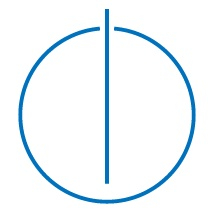
\includegraphics[width=0.2\linewidth]{figures/infologo.jpg}
	\end{figure}
	\bigskip 
\end{center}
\vfill

\newpage
\setcounter{page}{1}
\hoffset=0mm
\bibliographystyle{wmaainf} % quotation style
\setcounter{tocdepth}{3}
\setcounter{secnumdepth}{3}
\fboxsep 0mm

\tableofcontents

\newpage
\setlength{\baselineskip}{3ex}

\begin{spacing}{1.15}
	\chapter{Einleitung}
Im Verlauf der letzten 20 bis dreißig Jahre haben Computer das Leben der Menschheit entscheidend beeinflusst. In der Berufswelt ist der PC schon seit langem nicht mehr wegzudenken, aber auch im persönlichen Bereich sind sie weit verbreitet. Viele Haushalte besitzen schon einen oder mehr PCs und Laptops pro Person. Dank des rapiden Fortschritts werden Prozessoren nicht mehr nur in PCs eingesetzt, sondern auch in Autos und Smartphones. Mikrocontroller steuern heute fast alle alltäglichen technischen Geräte. Von der Waschmaschine über die Heizung zum Kühlschrank, alles wird gesteuert von einem kleinen Stück Silikon. Die ersten Schritte zu diesem Erfolg wurden in den späten 60er Jahren getätigt, als die ersten Mikroprozessoren entwickelt und veröffentlicht wurden. Ihre Neuerungen sowohl im Design als auch in der Produktionstechnik waren die Vorreiter für den jetzigen Erfolg. Deshalb werden hier zwei Chips vorgestellt, die beiden für sich beanspruchen der Erste gewesen zu sein. Der Intel 4004 wird von vielen als erster Mikroprozessor angesehen, während der TMS-1000 heute als erster Mikrocontroller betrachtet wird.
	\newpage
\section{Der Intel 4004}

Der 4004 ist der erste von Intel entwickelte Mikroprozessor und einer der Ersten überhaupt. Er gilt als einer der großen Meilensteine, die den Siegeszug der Computer einleitete. Schon Jahre vor seiner Entwicklung fingen Halbleiterchips an, die alten Elektronenröhren Rechner abzulösen. Durch die schnell voranschreitende Miniaturisierung von Transistoren ließen sich immer komplexere Logik Konstruktionen auf immer kleineren Chips umsetzen. Was vielversprechend begann, stellte sich allerdings bald als Problem heraus. Als die Komplexität und Spezialisierung einzelner Designs so stark zunahm, dass es nicht mehr kosteneffizient war manche Designs umzusetzen. Die Chips waren so spezialisiert geworden, dass die geringe Absatzmenge nicht die Entwicklungskosten rechtfertigte. Deshalb war es nur eine Frage der Zeit bis ein Universalrechner aus Silizium gebaut wurde. Deshalb beschäftigt sich der folgende Abschnitt mit der Geschichte des Intel 4004 und den Personen, die maßgeblich zu seiner Entwicklung beigetragen haben.
 
\subsection{Die Geschichte und Entwicklung des 4004}

Als im Sommer 1969 Busicom, ein japanischer Hersteller von elektrischen Rechenmaschinen, das Unternehmen Intel damit beauftragte die Chips für ihre neue Reihe von Rechenmaschinen zu produzieren, war Intel gerade mal ein Jahr alt. Das Unternehmen war spezialisiert auf die Herstellung von Halbleiter Speicherchips und hatte zum Zeitpunkt des Auftrags nur zwölf Mitarbeiter. Intel war zu dieser Zeit, auf Grund von fehlenden Absatzzahlen ihrer Speicherchips, in einem finanziellen Engpass und sah sich gezwungen die Arbeit anzunehmen.
\vspace{-24pt}
\begin{wrapfigure}{r}{0.6\textwidth}
	\vspace{20pt}
	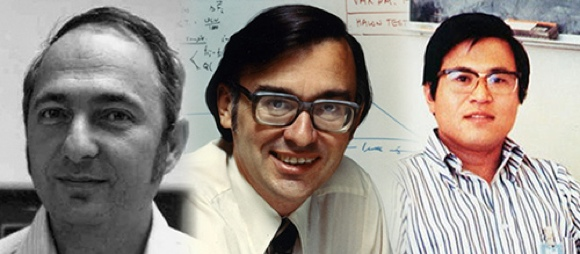
\includegraphics[width=0.6\textwidth]{figures/creators1.jpeg}
	\caption{v.l.n.r Mazor, Hoff und Shima}
	\label{fig:creators1}
	\vspace{-20pt}
\end{wrapfigure}

Busicom hatte schon einen großen Teil der Designarbeit getan und schickte drei Mitarbeiter zu Intel nach Kalifornien um die Arbeit zu vollenden und sie Intel zu übergeben.
Unter ihnen befand sich auch Masatoshi Shima, der eine wichtige Rolle in der Entwicklung des Intel 4004 spielen sollte. Als Kontaktpersonen wurde von Intel Marcian Edward "Ted" Hoff, Jr. und Stanley "Stan" Mazor abgestellt. Hoff, der in den Jahren bevor er zu Intel wechselte, in Stanford während seiner Forschung schon viele Arten von Computern studiert hatte, konnte sein persönliches Interesse nicht zurückhalten und studierte die Designpläne Busicoms. Der Plan von Busicom umfasste sieben Chips mit den speziellen Aufgaben: Programmkontrolle, Dezimalarithmetik, Timing, Read-Only-Memory, Schieberegister, Druckerkontrolle und Output Ports. Das ROM sollte zur Speicherung von Makroinstruktionen dienen, während die Schieberegister für den Datenspeicher genutzt werden sollten. Die Schieberegister wurden damals häufig verwendet, denn sie waren schnell für arithmetische Berechnungen und Ein- und Ausgabe Operationen. Problematisch hingegen waren das komplexe Timing und die langsamen Zugriffszeiten bei random access. Ein anderes Problem dieses ersten Designentwurfs war der komplexe Befehlssatz. Er bestand aus Makroinstruktionen, die viel fest verdrahtete Logik auf den Chips benötigten.
Nachdem er das Design analysiert hatte, befand Hoff, dass es nur für Busicom Rechenmaschinen einsetzbar sein würde und damit für Intel nicht kosteneffizient sein würde. Auch hatte Intel zu diesem Zeitpunkt weder die nötigen Logikdesigner noch die Produktionsmöglichkeiten von Chips dieser Komplexität. Als Hoff der Führungsebene von Intel deshalb einen alternativen Vorschlag machte, waren sie sehr offen und ermutigten ihn sein Design weiterzuentwickeln.
\newline
\vspace{-23pt}
\begin{wrapfigure}{hr}{.5\textwidth}
	\vspace{-5pt}
	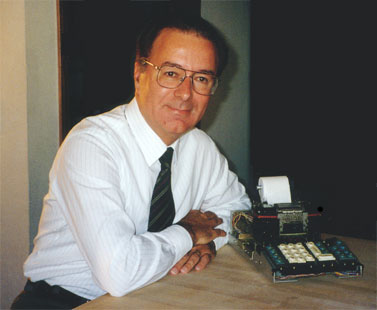
\includegraphics[width=0.5\textwidth]{figures/faggin.jpg}
	\caption{Federico Faggin}
	\label{fig:creators2}
	\vspace{-5pt}
\end{wrapfigure} 

Eine der großen Änderungen, die Ted Hoff vorschlug, war das Aufbrechen von Makroinstruktionen in kleinere, elementare Mikroinstruktionen. Die alte Funktionalität ließe sich als Subroutine in einem Programm implementieren. Das erhöhte zwar den Speicherverbrauch für Programmcode,
vereinfachte allerdings die Logik und war ein erster Schritt zu einem universal
einsetzbaren Prozessor. Schon vorher sollten die Befehle aus einem ROM gelesen werden, die Schieberegister für wieder beschreibbaren Speicher wurden allerdings durch bei Intel entwickelte dynamische RAMs ersetzt. Diese hatten den selben Platzverbrauch wie Schieberegistern, waren bei zufälligen Speicherzugriffen aber weit aus schneller. Dadurch entstand auch, der Vorschlag drei Chips zu designen. Eine CPU für die Berechnungen, und zwei erweiterbare Speicher für Programm- und Datenspeicherung. Zusätzlich wurde ein weiterer Chip entworfen, der die Ein- und Ausgabe Möglichkeiten erweitern sollte. Das System dieser vier Chips wurde MCS-4 genannt.
Eine Abschätzung des Designteams um Hoff, Mazor und Shima betrug 1900 Transistoren pro Chip, womit es bei weitem kostengünstiger als das währenddessen verbesserte Busicom Design war.
Dieses enthielt nämlich immer noch 12 Chips mit jeweils 2000 Transistoren und 40 Pins.
Die Einfachheit und die Flexibilität des neuen Chips waren Gründe, weshalb sich Busicom Ende 1969 dafür entschied mit dem Vorschlag von Intel weiterzumachen anstatt das eigene Design weiter zu verfolgen. 
Für das Logik- und Chipdesign wurde Anfang 1970 Federico Faggin eingestellt. Er sollte zusammen mit Shima innerhalb von 6 Monaten eine getestete Logikschaltung entworfen und diese in einem integrierten Schaltkreis umgesetzt haben. Währenddessen würde
 \newline
 \vspace{-24pt}
 \begin{floatingfigure}[l]{.5\textwidth}
 	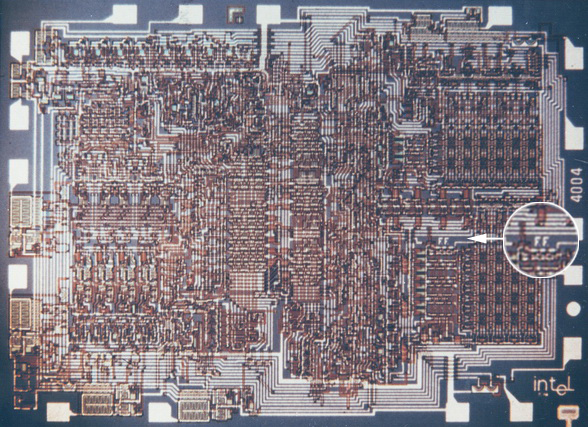
\includegraphics[width=0.5\textwidth]{figures/circuit.jpg}
 	\caption{Intel 4004 mit Faggins Initialen}
 	\label{fig:circuit}
 \end{floatingfigure} 
Shima an den Programmen für den neuen Prozessor arbeiten.
Nach 9 Monaten harter Arbeit hatte Faggin es geschafft und es lagen die ersten funktionsfähigen Prototypen des Chips vor.
Nach dem beheben einiger kleiner Fehler wurden die Chips an Busicom geliefert und wie geplant in den Rechenmaschinen eingesetzt. Einer der ersten Rechner, der das MCS-4 benutzte war der Busicom 141-PF. Er enthielt den 4004, 4 ROM-Chips mit dem Schon im Sommer 1971 kam
 Busicom allerdings erneut auf Intel zu um die Produktionskosten der Chips zu reduzieren. Auf Grund von steigender Konkurrenz und fallenden Preisen war Busicom nicht mehr konkurrenzfähig und in finanziellen Problemen. Nach langen Diskussionen der Intel Führungsebene entschloss sich das Unternehmen auf Grund des vielfältigen Einsetzbarkeit des Prozessors die Rechte an dem Prozessor von Busicom für {\$}60.000 zurückzukaufen. So konnte Intel im Frühjahr 1971 die Chipreihe auf den Markt bringen und so der Öffentlichkeit zugänglich machen. Währenddessen lief schon die Entwicklung des Intel 8008, des ersten Intel 8-Bit Prozessors. Dieser profitierte klar von dem Design des 4004 und führte später zu Intels Erfolg.
 
\subsection{Die Architektur des MCS-4}
Unter dem MCS-4 veröffentlichte Intel in 1971 eine Sammlung von vier Chips. Die Chips waren durchnummeriert von 4001 bis 4004 und stellten den ersten Universalcomputer auf Halbleiterbasis da. Das minimale System besteht aus nur einer CPU, dem 4004 und einem ROM. Es können allerdings bis zu 16 ROM und 16 RAM Chips angeschlossen werden. Verbunden werden diese Chips über einen 4 Bit breiten Bus. Der Prozessor kann zudem die anderen Chips durch Kontrollleitungen steuern. Als Schaltungskonzept wurde eine Mischung aus von Neumann und Harvard Architektur umgesetzt. Eigentlich Konkurrenzarchitekturen vereint das MCS-4 Ansätze von beidem, in dem es wie in der Harvard Architektur üblich Programm- und Datenspeicher trennt, aber trotzdem beide Speicher über den selben Bus angeschlossen sind. Dadurch lassen sich Befehle und Daten nur sequentiell anstatt parallel laden. Die folgenden Abschnitte befassen sich mit dem Aufbau der einzelnen Chips.

\subsubsection{Der 4001}
 \begin{floatingfigure}[r]{.5\textwidth}
 	\vspace{-10pt}
 	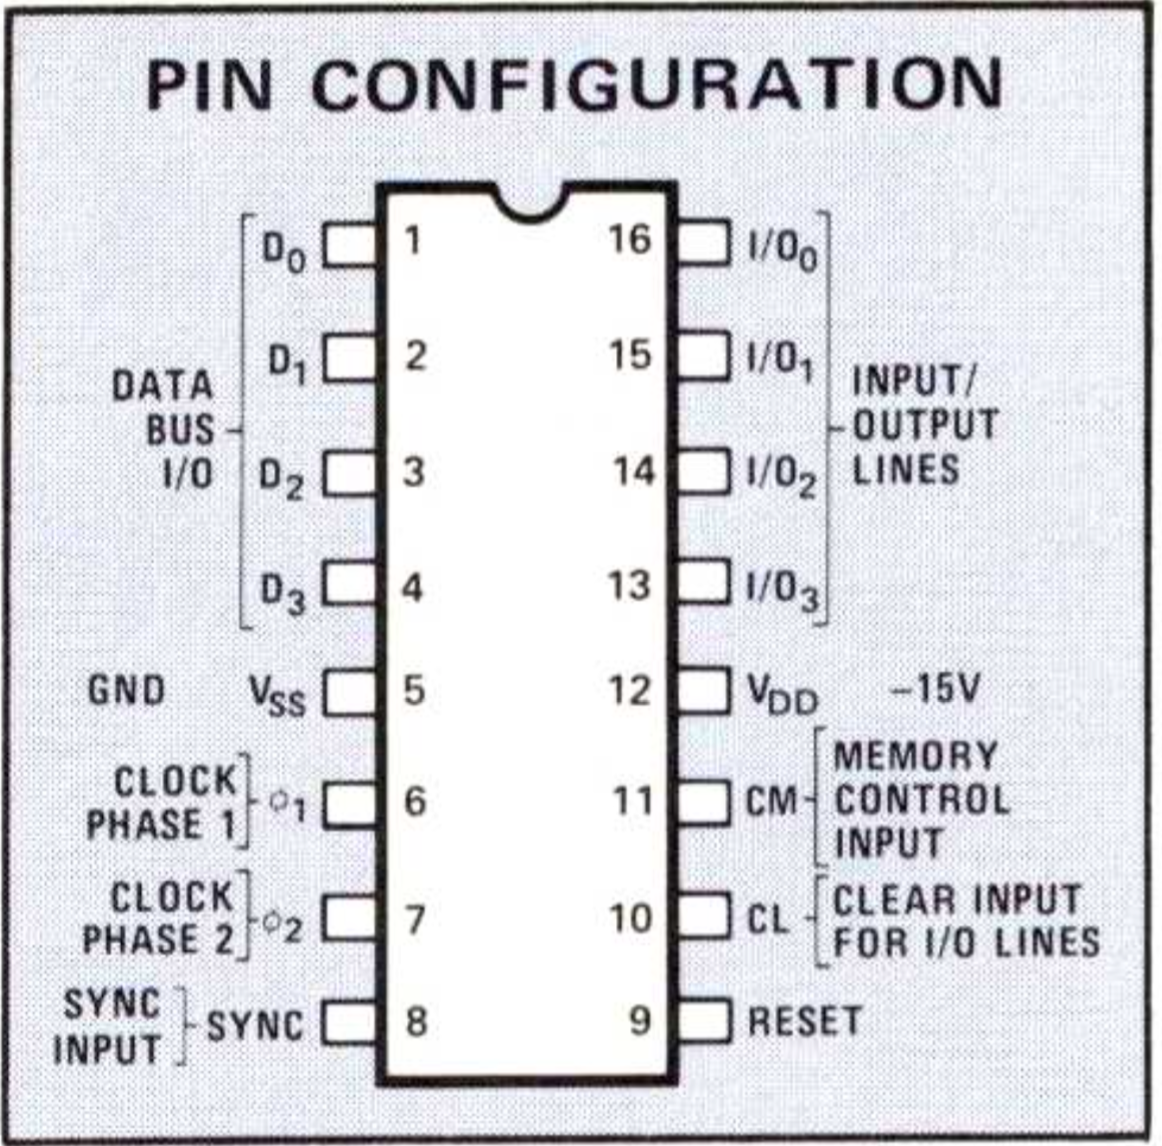
\includegraphics[width=0.5\textwidth]{figures/pins_4001.png}
 	\caption{Pins des Intel 4001}
 	\label{fig:pins_4001}
 \end{floatingfigure}
 Der 4001 ist ein programmierbarer Read-Only-Memory Chip. Er wird hauptsächlich dazu benutzt die Programmbefehle zu speichern. Dafür können im MCS-4 System bis zu 16 ROMs gleichzeitig angeschlossen werden. Pro Chip stehen dabei jeweils 2048 Bit zur Verfügung. Aufgeteilt sind diese in 256 Wörter mit jeweils 8 Bit. Der Chip besitzt 16 Pins über die Datenleitungen und Kontrollsignale angeschlossen werden. In \ref{fig:pins_4001} werden diese dargestellt. Die Pins $D_0$ bis $D_3$ sind die vier Datenleitungen, über die der 4 Bit breite Datenbus angeschlossen wird. Dieser Bus verbindet alle angeschlossenen 4001, 4002 und 4004 Chips. Über ihn werden die Speicheradressen vom Prozessor an das ROM geschickt. Daraufhin sendet das ROM die in der adressierten Speicherzelle enthaltene Instruktion zurück. Die Pins 5 und 12 werden mit den Versorgungsspannungen verbunden. Damit wird der Chip mit Energie versorgt. $V_{SS}$ ist äquivalent zu GND, während an $V_{DD}$ eine Spannung von $-15V$ anliegt.
 An den Pins 6 und 7, bezeichnet mit $\phi_1$ und $\phi_2$, werden zwei Taktsignale angeschlossen. Diese dienen der Synchronisation der Aktionen mehrerer Schaltkreise. In jedem Takt ist es für jeden Schaltkreis möglich eine Aktion auszuführen. Das SYNC-Signal, ist auch eine Art Takt und dient zur Synchronisation eines Befehlszyklus. Ein Zyklus besteht aus mehreren Takten der $\phi_1$ und $\phi_2$ Signale. Diese drei Signale sorgen für das Timing in allen Chips. Das CM-Signal auf Pin 11 wird dazu verwendet um einem adressierten Chip zu signalisieren, dass er in den nächsten zwei Zyklen auf den Bus schreiben darf. Das Reset-Signal löscht alle internen Register, mit der Ausnahme der Input und Output Register.
 \begin{figure}[h]
 	\centering
  	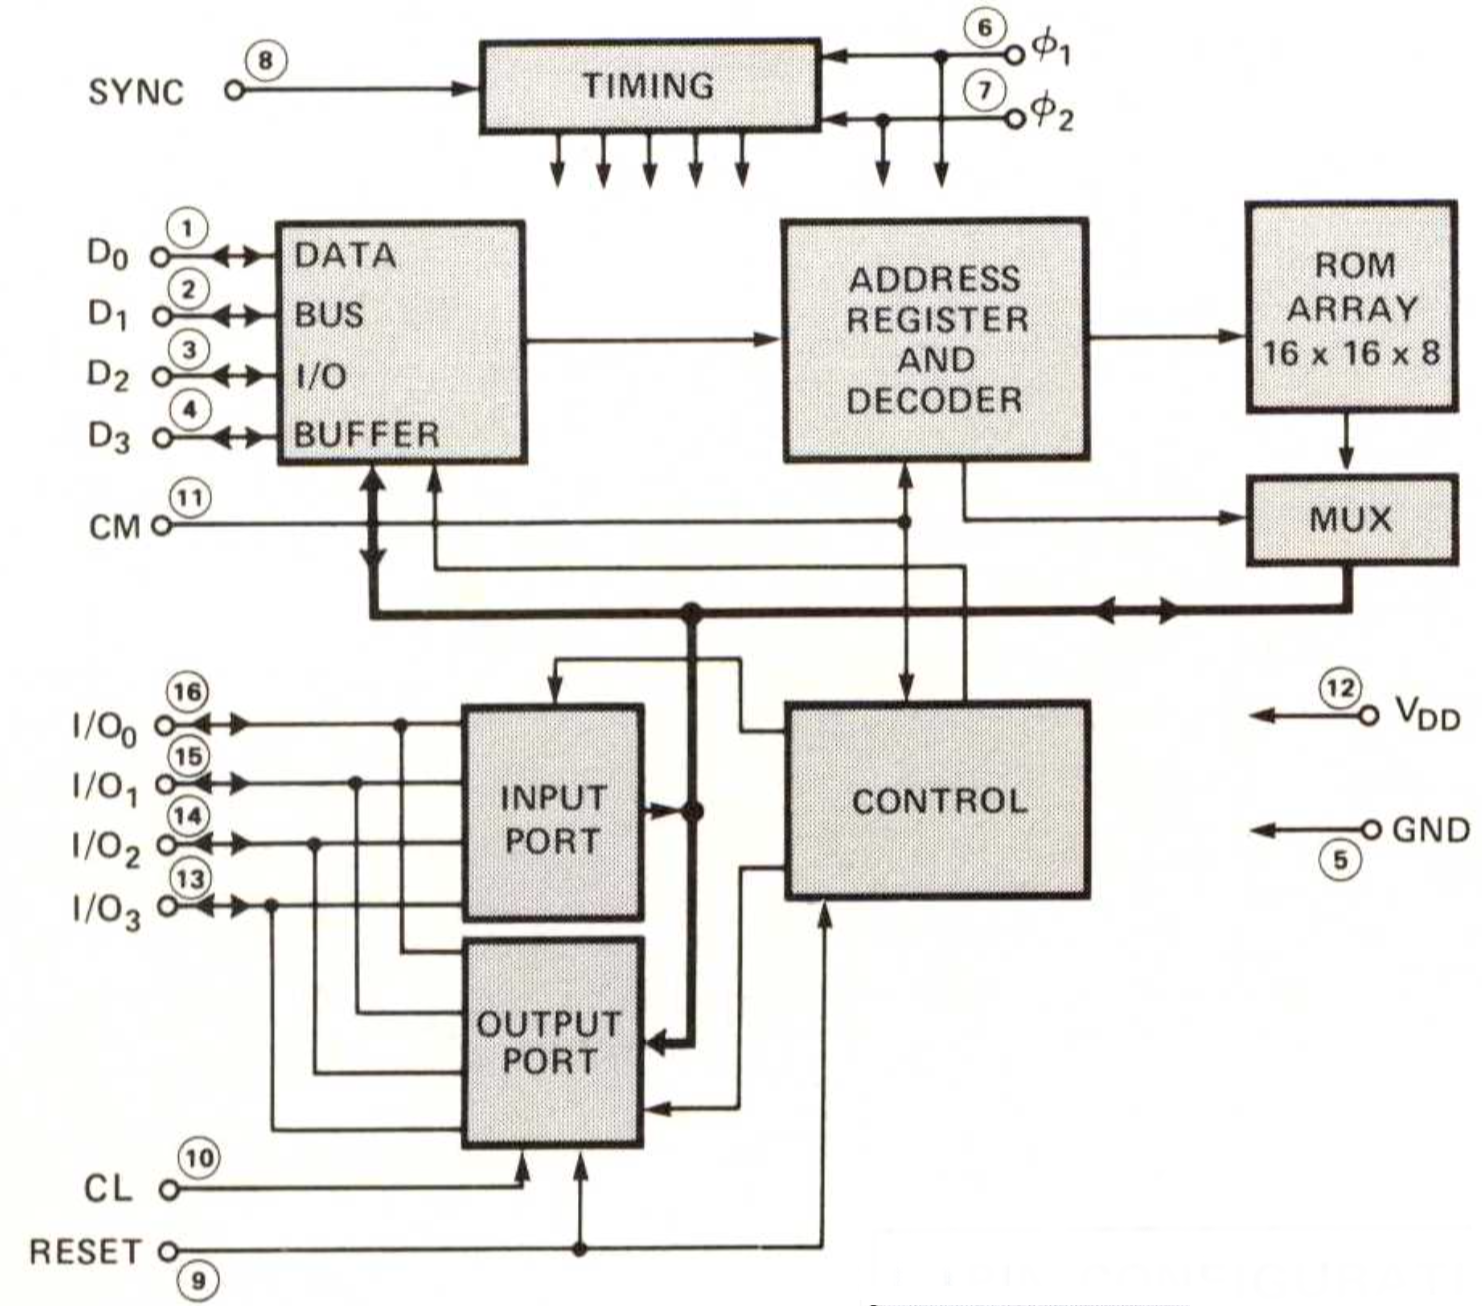
\includegraphics[width=0.8\textwidth]{figures/layout_4001.png}
  	\caption{Layout des Intel 4001}
  	\label{fig:layout_4001}
 \end{figure}
Diese werden über das Clear-Signal gelöscht. Die Ein- und Ausgaberegister sind Teil der zweiten Funktionalität des Intel 4001. In seiner zweiten Funktion kann es auch als Schnittstelle zu Peripheriegeräten dienen. Dazu gibt es 4 weitere Leitungen an den Pins 13 - 16. In \ref{fig:layout_4001} ist zu sehen,dass es möglich ist jeden Pin individuell als Input oder als Output Port zu definieren. Über den internen Bus des 4001 werden Daten entweder direkt zu den I/O-Registern geliefert, oder wenn eine Adresse am Bus anliegt im Adressregister gespeichert. Nachdem die Adresse vollständig angekommen ist, wird sie dekodiert und die Instruktion aus dem ROM über einen Multiplexer wieder zurück auf den Datenbus geschrieben.

\subsubsection{Der 4002}
Der Intel 4002 ist das Gegenstück zu 4001. Während der eine die Programmdaten speichert, dient der 4002 als Datenspeicher. Im Vergleich zum 4001 besitzt dieser Chip weiter weniger Speicher. Nur 320 Bit stehen zur Verfügung aufgeteilt in 4 Register. Jedes dieser Register besteht aus 20 4-Bit Wörtern. Davon können 16 zum speichern von Daten
\vspace{-23pt}
 \begin{floatingfigure}[r]{.5\textwidth}
 	\vspace{-10pt}
 	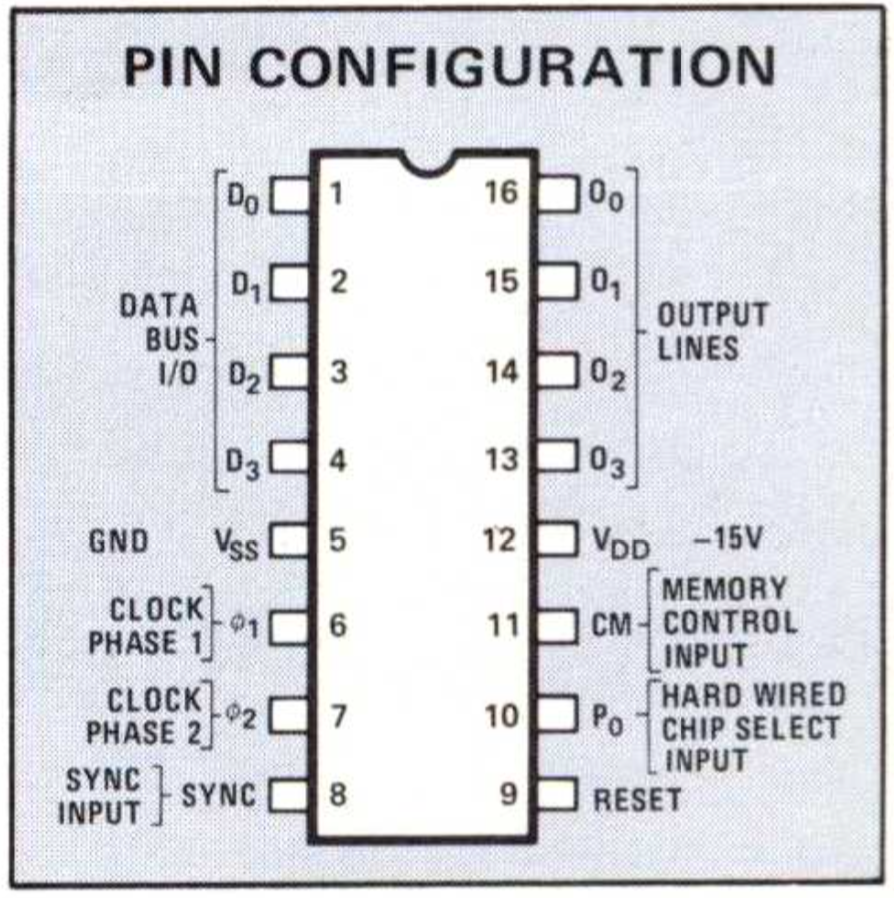
\includegraphics[width=0.5\textwidth]{figures/pins_4002.png}
 	\caption{Pins des Intel 4002}
 	\label{fig:pins_4002}
 \end{floatingfigure}
verwendet werden, während die letzten 4 als Registerstatusbits benutzt werden. Auch hier kann die Speichergröße wieder durch das Anschließen von bis zu 16 Chips erhöht werden. Wie der 4001 ist auch der RAM-Chip über den Datenbus mit den anderen Chips verbunden. Ebenso identisch sind die Timing Logik und Spannungsversorgung. Der erste Unterschied in der Pinbelegung ist der $P_0$ Eingang. Der 4002 kommt in zwei verschiedenen Ausführungen: 4002-1 und 4002-2. Diese sind von der Logik identisch, haben jedoch eine andere Verdrahtung. Das führt dazu, dass pro CM-Signallinie des Prozessors nur vier 4002 Chips angeschlossen werden können. Pro Signallinie genau 2 von jeder Sorte.
Damit ergeben sich folgende Adressen für die vier Chips an einer Signallinie:
\begin{table}[H]
	\centering
	\begin{tabular}{c | c | c | c  c}
		Chipnummer & 4002 Option & $P_0$ & $D_3$ & $D_2$ \\
		\hline
		0 	& 4002-1 & GND & 0 & 0 \\
		1	& 4002-1 & $V_{DD}$ & 0 & 1 \\
		2	& 4002-2 & GND & 1 & 0 \\
		3	& 4002-2 & $V_{DD}$ & 1 & 1	
	\end{tabular}
	\caption{RAM-Chipauswahl}
	\label{ramauswahl}
\end{table}

$P_0$ kann fest verdrahtet werden und ist eine zusätzliche Möglichkeit einen Chip auszuwählen. Wenn Daten aus dem RAM geladen werden sollen geschieht das in zwei Befehlszyklen. Im ersten wird die Adresse an den RAM Chip gesendet und im zweiten die Daten zurück an den Prozessor.
\begin{table}[H]
	\centering
	\begin{tabular}{c | c | c | c}
		\multicolumn{2}{c|}{X2} & \multicolumn{2}{c}{X3} \\
		\hline
		$D_3$ \space\space\space $D_2$ & $D_1$ \space\space\space $D_0$ & $D_3$ \space\space\space $D_2$ & $D_1$ \space\space\space $D_0$ \\
		Chip {\#} & Register {\#} & \multicolumn{2}{c}{Speicherzelle}
	\end{tabular}
	\caption{RAM-Adressierung}
	\label{ramadresse}
\end{table}
Die Adressenübertragung findet in zwei Schritten statt, siehe \ref{ch:befehlszyklus}.
Im ersten Schritt X2 wird die Chipnummer und die Registernummer verschickt. 
Im zweiten die Adresse einer der 16 Speicherzellen innerhalb des Registers.
Dabei sind D0 - D3 die vier Bits die gleichzeitig auf den 4 Datenbuslinien liegen. Befinden sich die gesuchten Daten nicht auf einem der 4 Chips der aktuell ausgewählten RAM-Bank, so muss vor der Adressenübertragung die Bank in einem extra Befehlszyklus gewechselt werden. Als RAM-Bank wird eine Kombination von bis zu vier RAM-Chips genannt, die an der selben CM-Signallinie liegen. Mit Hilfe des designate-command-line Befehls wird eine CM-Linie ausgewählt. Wie bei den 4001 Chips gilt auch hier, dass ein Chip nur Daten vom Bus empfängt, wenn seine CM-Linie aktiviert wird.
 \begin{figure}[h]
 	\centering
 	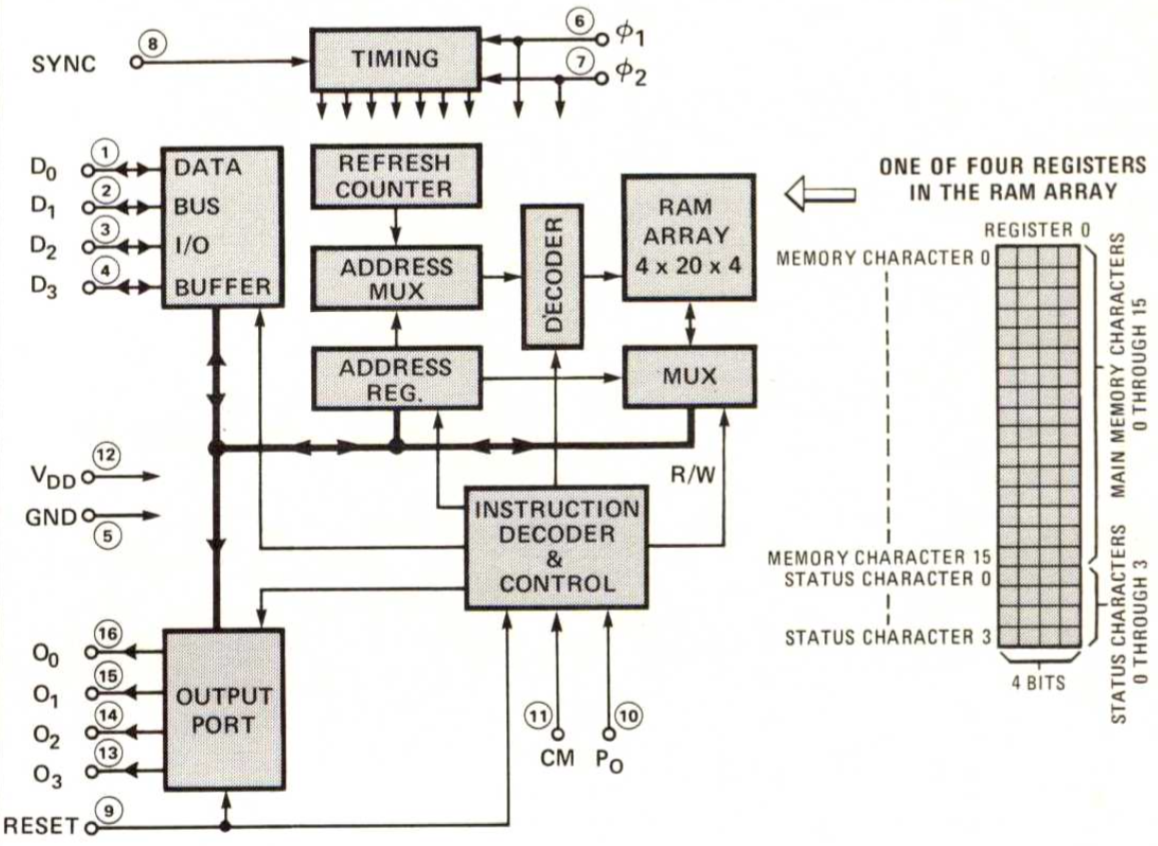
\includegraphics[width=0.9\textwidth]{figures/layout_4002.png}
 	\caption{Layout des Intel 4002}
 	\label{fig:layout_4002}
 \end{figure}
 
 Nachdem die Adresse angekommen ist, wird sie wie beim 4001 in einem Adressenregister zwischengespeichert und dekodiert. Danach wird im nächsten Befehlszyklus der Wert der entsprechenden Speicherzelle auf den Datenbus gelegt. Wie der Intel 4001 besitzt auch der 4002 4 Output Pins. Auch hier können Peripheriegeräte angeschlossen werden. Alle Register sowie der Speicher werden gelöscht wenn das Reset-Signal für mehr als 32 Befehlszyklen aktiviert wird.

\subsubsection{Der 4003}
 \begin{floatingfigure}[r]{.5\textwidth}
 	\vspace{-10pt}
 	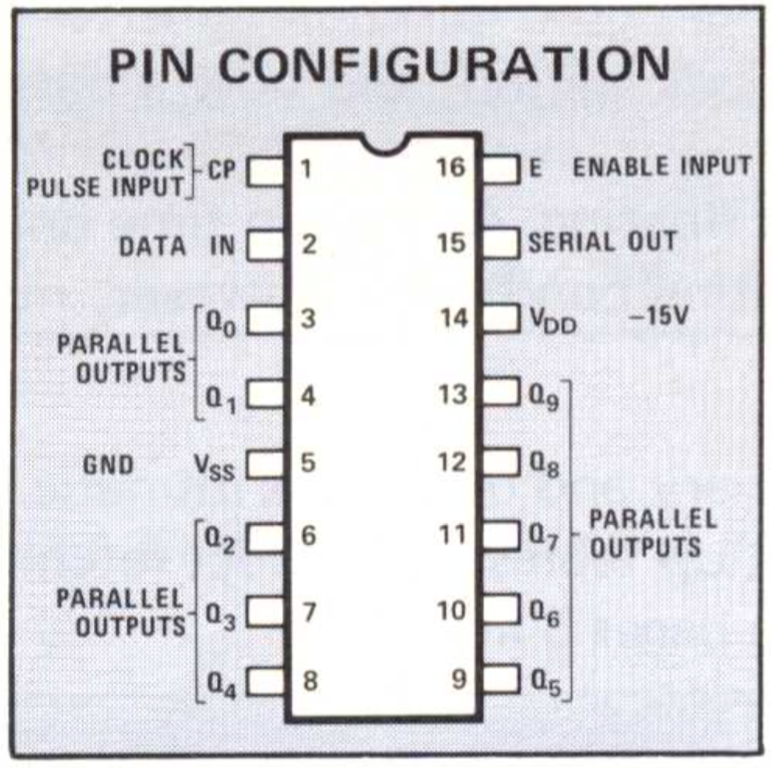
\includegraphics[width=0.5\textwidth]{figures/pins_4003.png}
 	\caption{Pins des Intel 4003}
 	\label{fig:pins_4003}
 \end{floatingfigure}
Der dritte Chip aus der Reihe ist Intel 4003. Er besteht hauptsächlich aus einem 10 Bit Schieberegister. Der Chip wurde entworfen um die Ein- und Ausgabemöglichkeiten des Systems zu erweitern. Während der 4002 schon über Ausgabe und der 4001 sowohl über Aus- als auch Eingabe Möglichkeiten verfügt, gibt es immer noch Fälle in denen diese Pins nicht ausreichen. Deshalb können die 4003 Chips an diese Pins angeschlossen werden. Über den Serial-Input Pin wird das Schieberegister mit Daten befüllt. Über den CP-Pin wird das verschieben der Bits innerhalb des Registers gesteuert. Bei jeder Verschiebung wird das letzte Bit auf den seriellen Ausgang geschrieben. Die Daten aus dem Schieberegister können auch parallel ausgelesen werden. Dazu stehen 10 weitere Pins zur Verfügung.
 \begin{figure}[h]
 	\centering
 	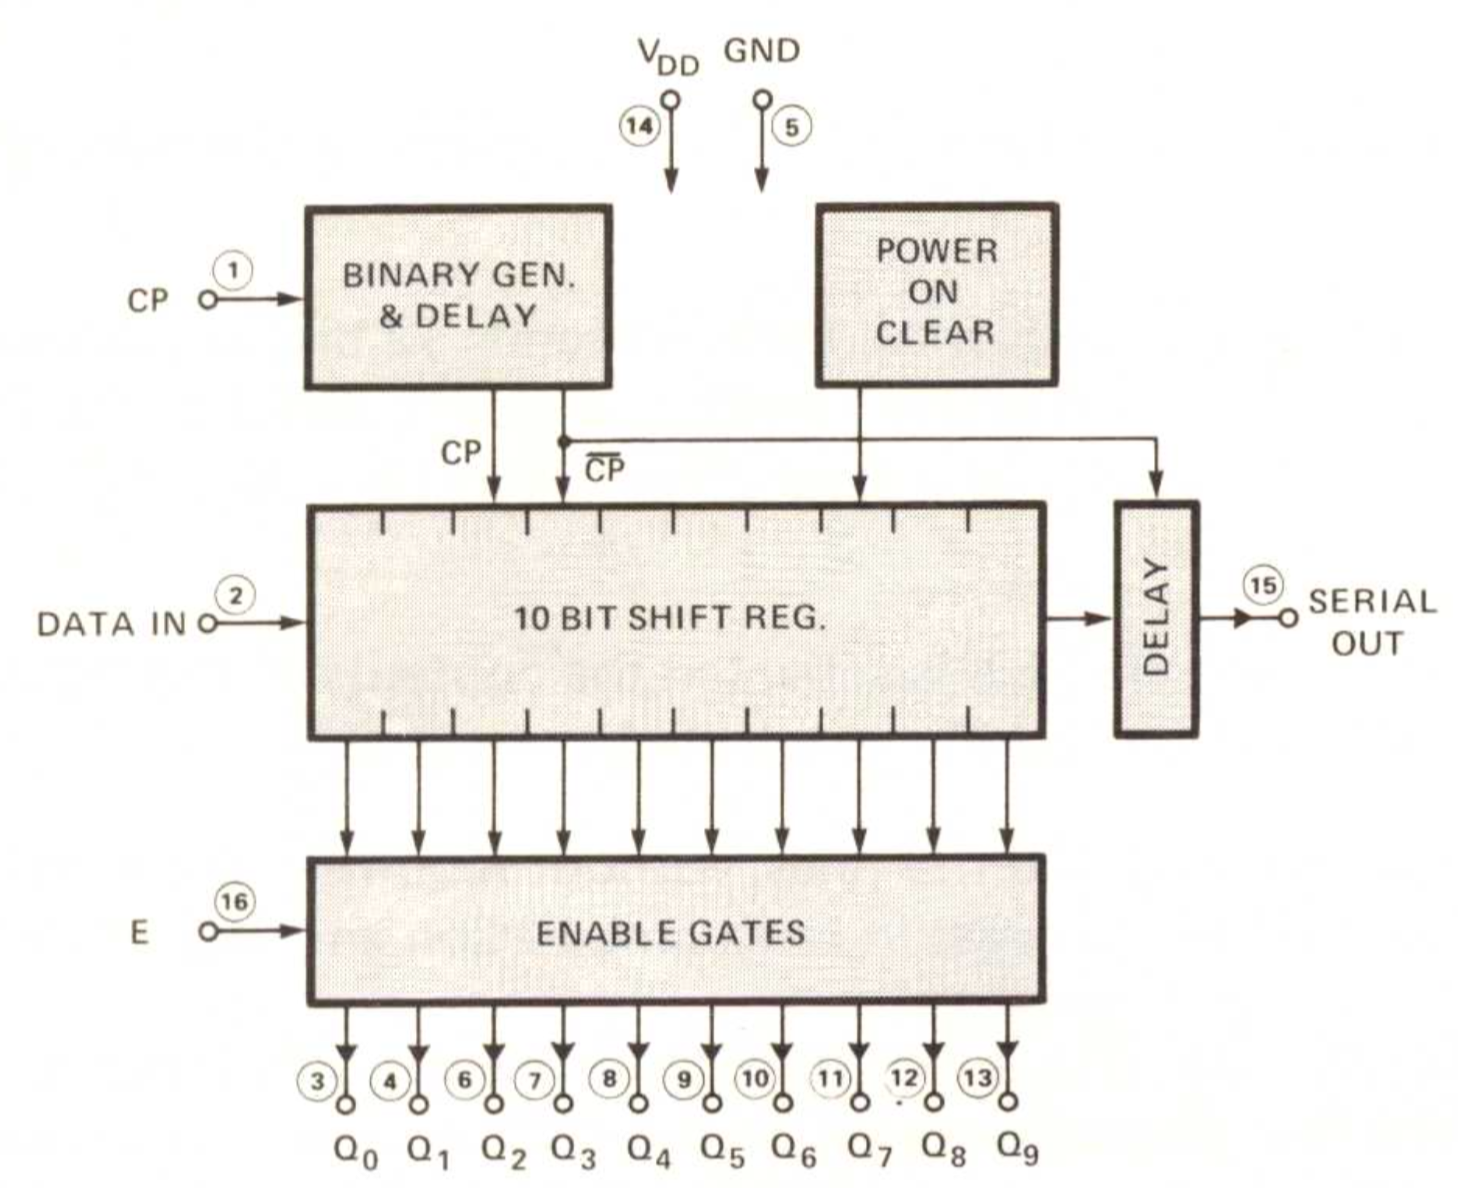
\includegraphics[width=0.7\textwidth]{figures/layout_4003.png}
 	\caption{Layout des Intel 4003}
 	\label{fig:layout_4003}
 \end{figure}
Die parallele Ausgabe wird mit Hilfe des Enable-Signal gesteuert. 
Wenn es aktiviert wird, werden alle 10 Bits gleichzeitig über die Pins $Q_0$ bis $Q_9$ ausgegeben. Um mehr Geräte wie Tastaturen, Displays oder Drucker anschließen zu können, können mehrere dieser Chips hintereinander geschaltet werden, so dass ein vielfaches der 10 Pins erreicht werden können.

\subsubsection{Der 4004}
 \begin{floatingfigure}[r]{.5\textwidth}
 	\vspace{-10pt}
 	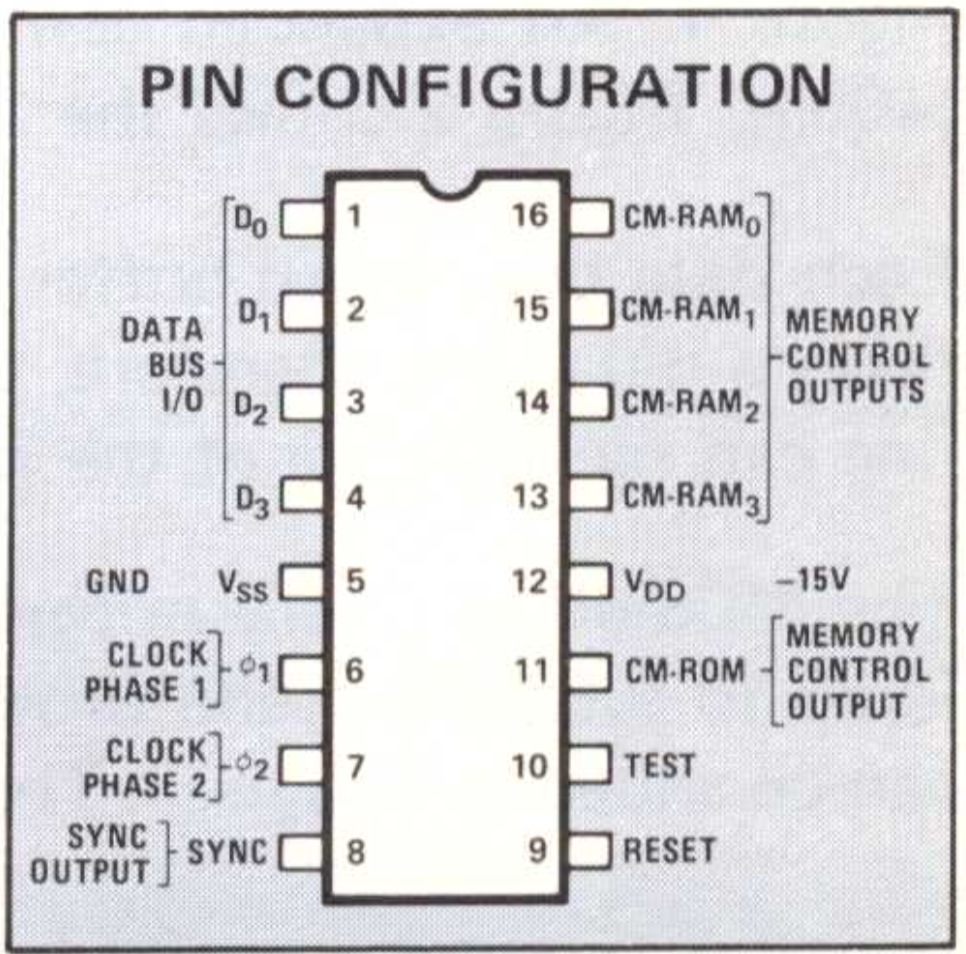
\includegraphics[width=0.5\textwidth]{figures/pins_4004.png}
 	\caption{Pins des Intel 4004}
 	\label{fig:pins_4004}
 \end{floatingfigure}
Der Intel 4004 ist das Kernstück des Systems. Der Chip ist eine CPU und wurde entworfen um mit den anderen Chips zusammenzuarbeiten und sie zu steuern. Er bearbeitet die Befehle, welche im 4001 ROM gespeichert sind. Dazu muss müssen die Befehle erst aus dem ROM geladen werden.
Dazu wird die Adresse über den Datenbus an die ROMs verschickt und das CM-ROM Signal aktiviert. Wenn der aktuelle Befehl geladen wurde, wird er im Instruktionsregister gespeichert. Das Register besteht aus zwei 4 Bit Wörtern. Die ersten 4 geladenen Bit enthalten den Opcode und werden im OPR Teil des Registers gespeichert. Die zweiten Vier enthalten den Modifier. Er wird im OPA Teil des Registers gespeichert und enthält Adressen oder Daten, auf denen der Befehl ausgeführt wird. Direkt an das Register ist der Dekodierer angeschlossen, der die Instruktion dekodiert um sie ausführen zu können. Der zweite große Bestandteil des 4004 ist das Indexregister. Das Indexregister ist ein interner Cache zur Speicherung von Zwischenergebnissen und Instruktionen. Dazu können die 64 Bit auf zwei verschiedene benutzt werden. Sie sind in 8 Reihen mit jeweils 8 Bit pro Reihe organisiert. Trotzdem können 16 verschiedene Zellen mit 4 Bit adressiert werden. Dadurch können sowohl 4 Bit Daten oder eine Reihe von 8 Bit als Instruktion oder Adresse ausgelesen werden. Das Adressenregister des Intel 4004 besteht aus 4 mal 12-Bit RAM. In einer dieser 12 Bit Speicherzellen liegt die aktuelle Programmadresse. Die zusätzlichen 3 Zellen werden benutzt um Adressen für Subroutinen zu speichern. Das bedeutet, dass bei der Programmierung des Prozessors bis zu 3 Subroutinen verschachtelt werden können.
Der vierte und letzte große Teil der CPU ist die ALU (Arithmetic Logical Unit). Die ALU besteht aus einem 4 Bit Addierer und einem Akkumulator inklusive eine Carry Flip-Flop. Der erste Term für die Addition/Subtraktion kommt aus einem Register, das über den internen Datenbus gefüllt wird. Der zweite Term kommt aus dem Akkumulator. Das Ergebnis der Berechnung wird wieder im Akkumulator gespeichert und das Carry-Bit gesetzt, falls ein Überlauf auftritt.
 \begin{figure}[h]
 	\centering
 	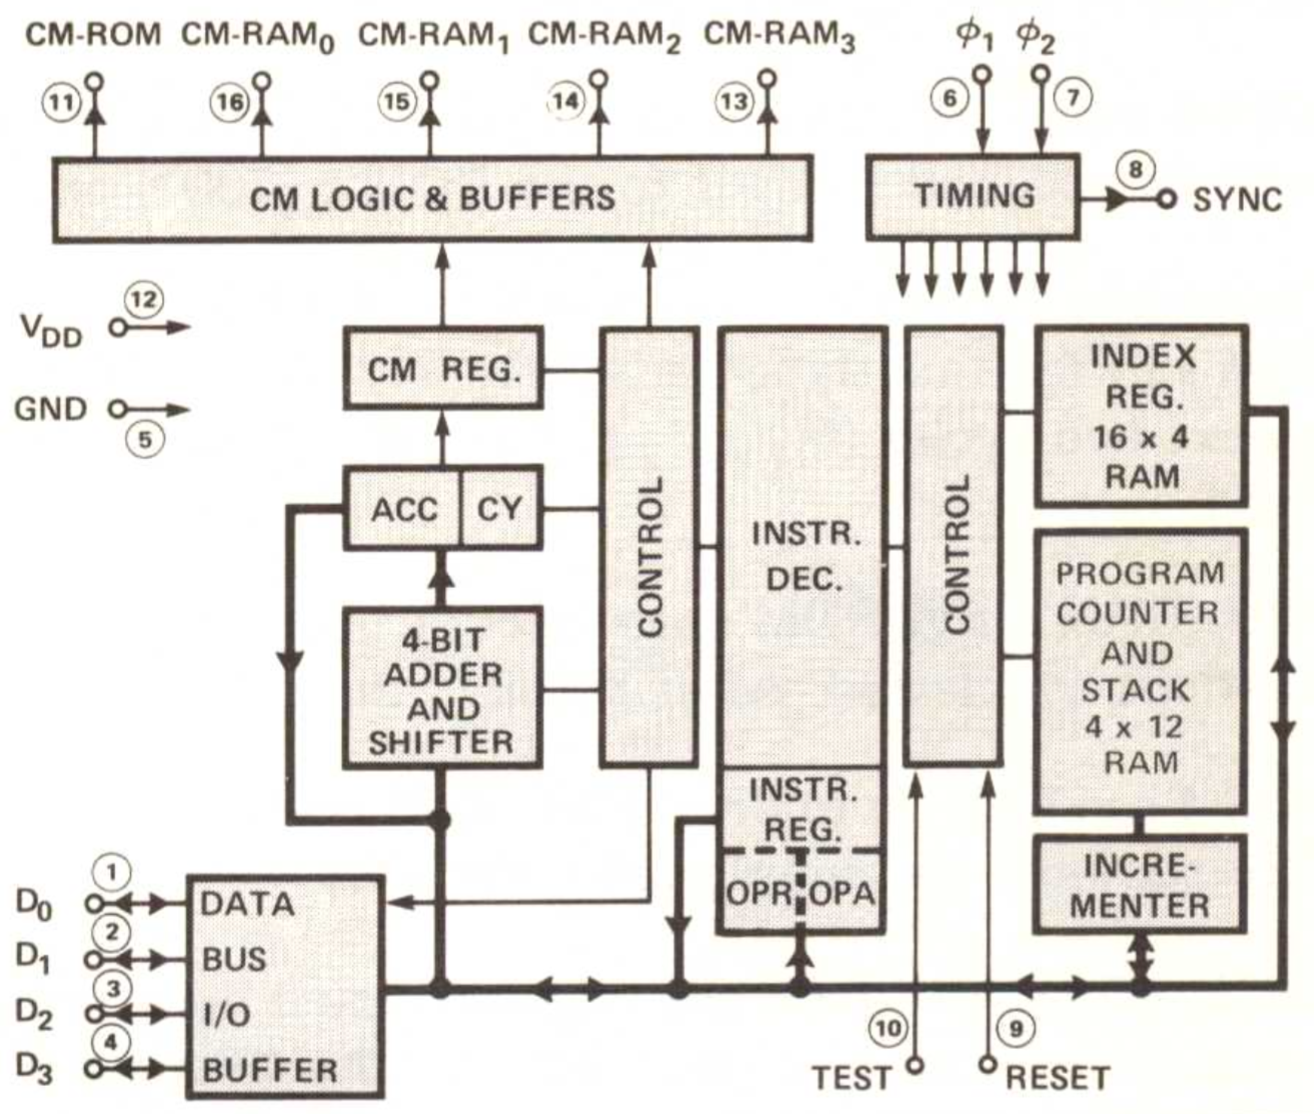
\includegraphics[width=0.7\textwidth]{figures/layout_4004.png}
 	\caption{Layout des Intel 4004}
 	\label{fig:layout_4004}
 \end{figure}
Die Berechnungen werden in Binärarithmetik ausgeführt. Es ist aber auch möglich einen \textit{Decimal Adjust} durchzuführen. Mit seiner Hilfe lassen sich Binärzahlen in so genannte Binary-Coded-Decimal Zahlen umwandeln. In dieser Art der Zahlendarstellung wird jede Dezimalstelle einer Zahl durch 4 Bit dargestellt. In diesen 4 Bit werden nur die Zahlen von 0-9 verwendet.

\subsection{Der Befehlszyklus}
\label{ch:befehlszyklus}

\subsection{Der Befehlssatz}
	\section{The TMS-1000}
\begin{frame}
	  \frametitle{Der erste Mikrocontroller - System-on-a-Chip}
	  \begin{center}

		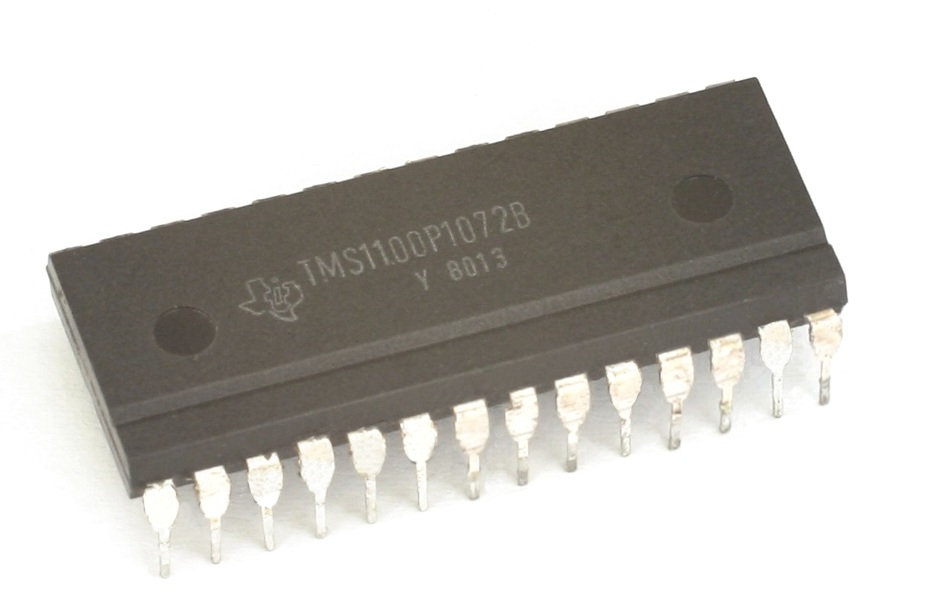
\includegraphics[scale=0.25]{images/KL_TI_TMS1100.jpg}


	  \end{center}
\end{frame}


\begin{frame}
	\frametitle{Inhalt}
		\begin{enumerate}
			\item Geschichte \pause
			\item Mikrokontroller allgemein \pause
			\item TMS1000 \pause \begin{itemize}
										\item Allgemeine Daten \pause
										\item Aufbau \& Funktionsweise \pause
										\item Befehlssatz \pause
										\end{itemize}
			\item Verwendung des TMS1000
		\end{enumerate}
\end{frame}

\subsection{Geschichte}
\begin{frame}
	\frametitle{Entstehung}
		\begin{itemize}
			\item Entwickelt von Gary Boone \& Michael Cochran 1971 \pause
			\item Zuerst von Texas Instrument verwendet \pause
			\item Erst 1974 auf dem freien Markt erh{\"a}ltlich \pause
			\item Bis heute ca. 100 Millionen verkaufte Exemplare 
		\end{itemize}
\end{frame}

\subsection{Mikrokontroller allgemein}
\begin{frame}
	\frametitle{Miktrokontroller allgemein}
		\begin{center}
		{\huge Aufbau:}
		\end{center}
		\begin{itemize}
		\item CPU - Prozessor \pause
		\item RAM - Arbeitsspeicher \pause
		\item ROM - Festspeicher \pause 
		\item Takt \pause
		\item Peripherie - I/O-Ports
		\end{itemize}
\end{frame}

\subsection{Der TMS-1000}
\begin{frame}
	\frametitle{Allgemeine Daten - TMS1000}
		\framesubtitle{Abbildung der Pins}
\begin{figure}
	\centering
		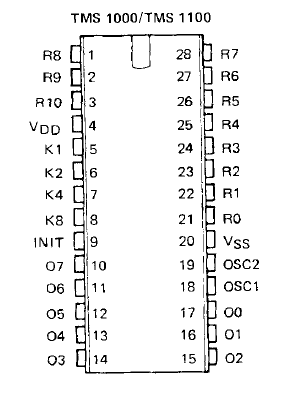
\includegraphics[scale=0.5]{images/pins.PNG}
\end{figure}

\end{frame}

\begin{frame}
	\frametitle{Allgemeine Daten - TMS1000}
	\begin{itemize}
		\item ROM: 1024x8 Bits \pause
		\item RAM: 64x4 Bits \pause
		\item 43 Basis Instruktionen \pause
		\item Max. Spannung 20V \pause
		\item H{\"o}chste erreichbare Frequenz: 0,4MHz
	\end{itemize}
\end{frame}


\begin{frame}
	\frametitle{Aufbau \& Funktionsweise}
		\framesubtitle{Schaltbild des TMS-1000}
\begin{figure}
	\centering
		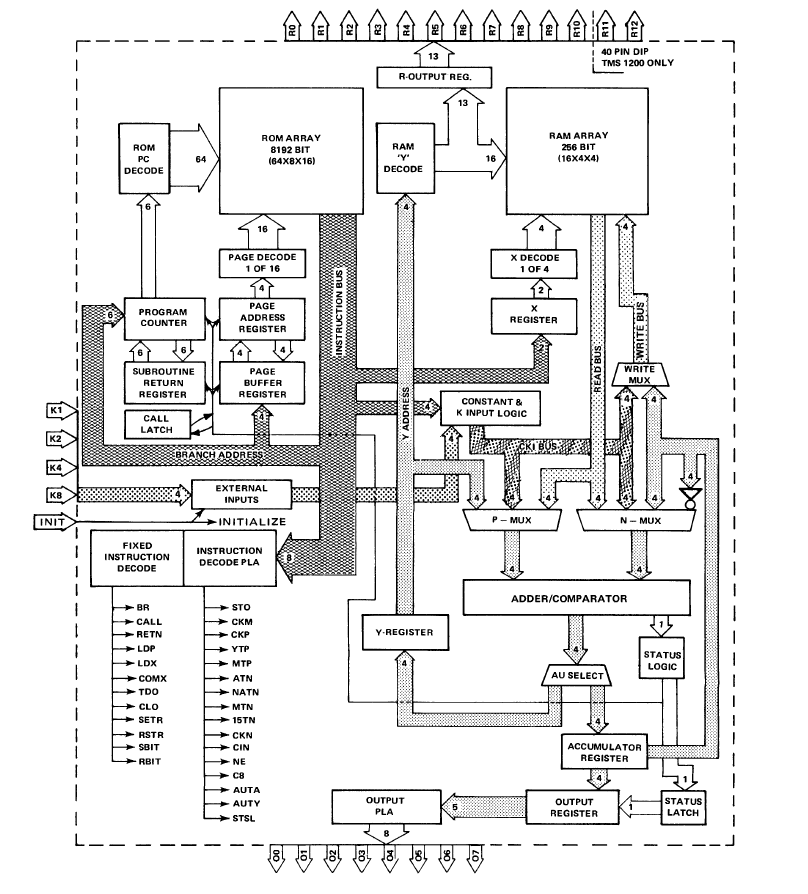
\includegraphics[scale=0.28]{images/schaltbild.PNG}
\end{figure}
\end{frame}

\begin{frame}
\frametitle{Aufbau \& Funktionsweise}
	  \framesubtitle{ROM}
		 \begin{columns}
      \begin{column}{5cm}
    		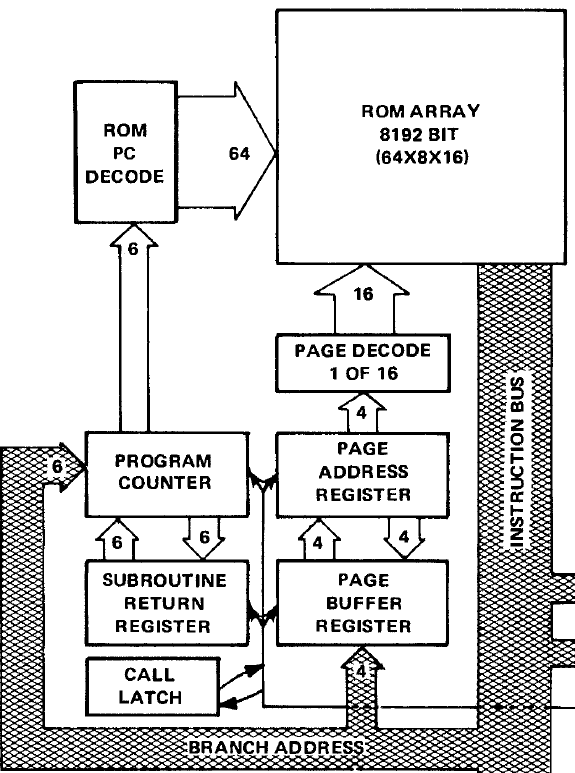
\includegraphics[scale=0.3]{images/ROM.PNG}
      \end{column}
      \begin{column}{5cm}
       \begin{itemize}
        \item 16 Seiten je 64 W{\"o}rter \pause
        \item 3 Register die den ROM adressieren \pause
        \item Page Adress (PA) \pause
        \item Page Buffer (PB) \pause
        \item Program Counter (PC)
       \end{itemize}
      \end{column}
     \end{columns}
\end{frame}

\begin{frame}
\frametitle{Aufbau \& Funktionsweise}
 \framesubtitle{Branching \& Subroutines}
 		 \begin{columns}
      \begin{column}{5cm}
    		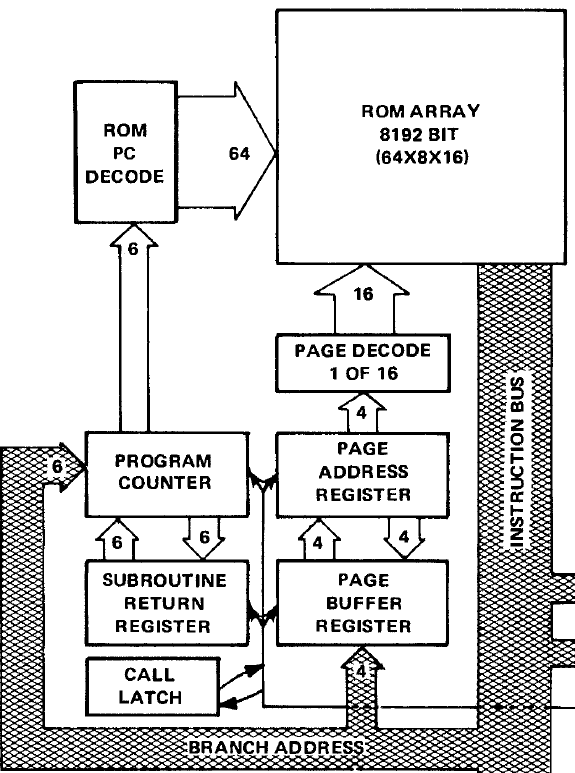
\includegraphics[scale=0.3]{images/ROM.PNG}
      \end{column}
      \begin{column}{5cm}
        	\begin{itemize}
 						\item Conditional \pause
 						\item ALU setzt Status-Logic Bit \pause
 						\item Standardm{\"a}{\ss}ig auf 1
 					\end{itemize}
      \end{column}
     \end{columns}
\end{frame}


\begin{frame}
\frametitle{Aufbau \& Funktionsweise}
	\framesubtitle{RAM}
		\begin{columns}
			\begin{column}{5cm}
				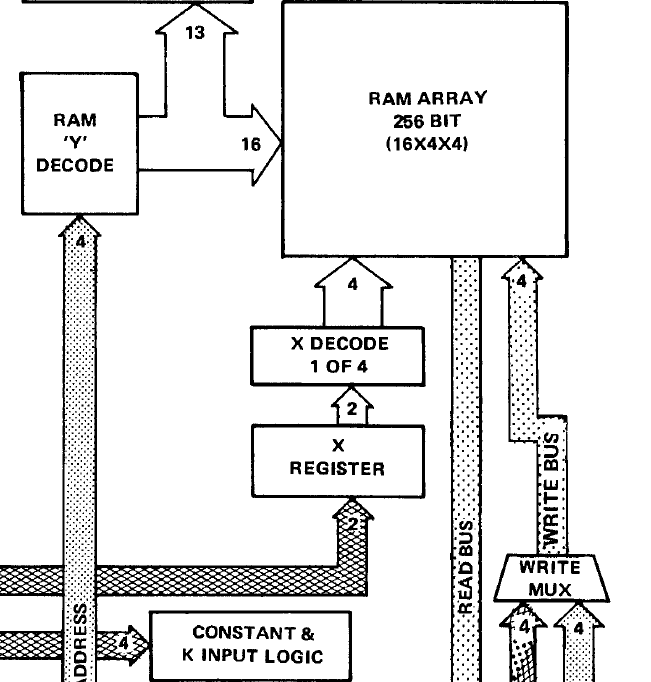
\includegraphics[scale=0.3]{images/RAM.PNG}
			\end{column}
			\begin{column}{5cm}
				\begin{itemize}
					\item 4 Dateien mit je 16 W{\"o}rtern \pause
					\item Wird durch X und Y Register adressiert \pause
					\item X adressiert "`Seite"', Y das Wort \pause
					\item Input durch Write-Multiplexer \pause
					\item Output durch Read-Bus
				\end{itemize}
			\end{column}
		\end{columns}
\end{frame}

\begin{frame}
\frametitle{Aufbau \& Funktionsweise}
	\framesubtitle{Constant and K Input (CKI) Logic}
		\begin{columns}
			\begin{column}{5cm}
				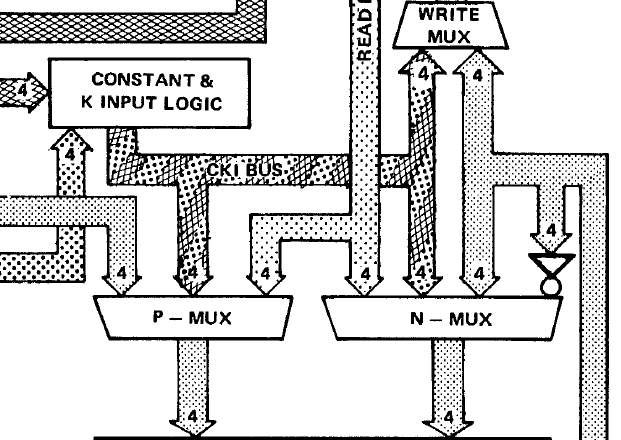
\includegraphics[scale=0.3]{images/CKI.PNG}
			\end{column}
		\begin{column}{5cm}
			\begin{itemize}
				\item Verwendet entweder K-Inputs oder Konstanten aus dem ROM \pause
				\item Kann entwededer in P-MUX, N-MUX oder RAM schreiben
			\end{itemize}
		\end{column}
	\end{columns}
\end{frame}


\begin{frame}
\frametitle{Aufbau \& Funktionsweise}
	\framesubtitle{Y-Register}
		\begin{itemize}
			\item Adressiert RAM \pause
			\item Setzt R-Output Latches
		\end{itemize}
\end{frame}


\begin{frame}
	\frametitle{R-Output}
		\begin{itemize}
			\item Externe Ger{\"a}te \pause
			\item	Display Scans \pause
			\item Input Encoding \pause
			\item Status Logic Outputs
		\end{itemize}
\end{frame}


\begin{frame}
\frametitle{Aufbau \& Funktionsweise}
	\framesubtitle{Akkumulator \& ALU}
		\begin{columns}
			\begin{column}{5cm}
				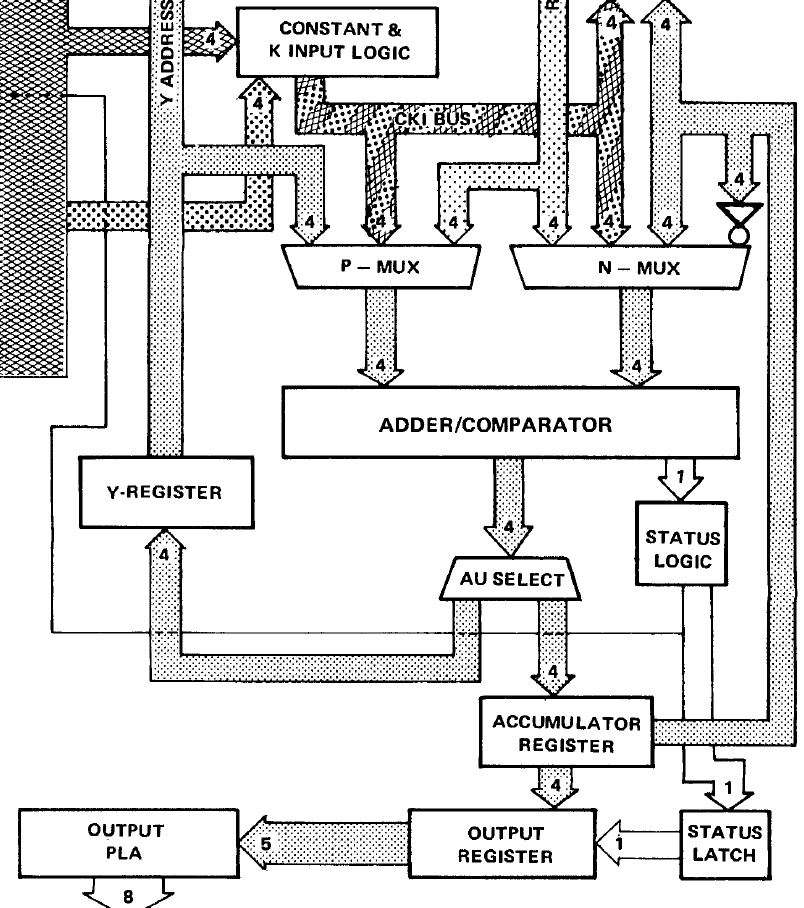
\includegraphics[scale=0.25]{images/ALU.PNG}
			\end{column}
			\begin{column}{5cm}
				\begin{itemize}
					\item 4-Bit Adder/Comperator \pause
					\item Kann addieren, subtrahieren und logische Vergleiche \pause
					\item Addition/Substraktion entweder im Y-Register oder Akkumulator gespeichert \pause
					\item Ergebnis Vergleiche im Status-Logic-Bit
				\end{itemize}
			\end{column}
		\end{columns}
\end{frame}
	

\begin{frame}
\frametitle{Aufbau \& Funktionsweise}
	\framesubtitle{O-Output}
		\begin{columns}
			\begin{column}{5cm}
				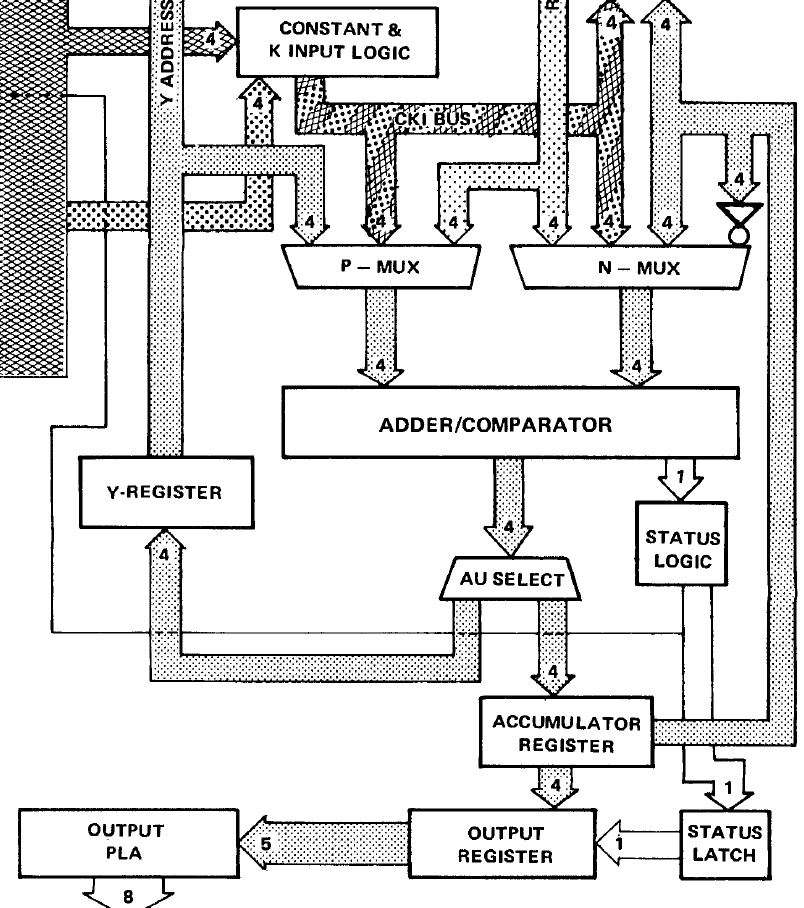
\includegraphics[scale=0.25]{images/ALU.PNG}
			\end{column}
			\begin{column}{5cm}
				\begin{itemize}
					\item Gibt Akkumulator und Status-Bit aus \pause
					\item PLA kodiert 5 Input-Bits in 8 Ausg{\"a}nge
				\end{itemize}
			\end{column}
		\end{columns}
\end{frame}

\begin{frame}
\frametitle{Aufbau \& Funktionsweise}
	\framesubtitle{Instruction-Decoder}
		\begin{columns}
			\begin{column}{5cm}
				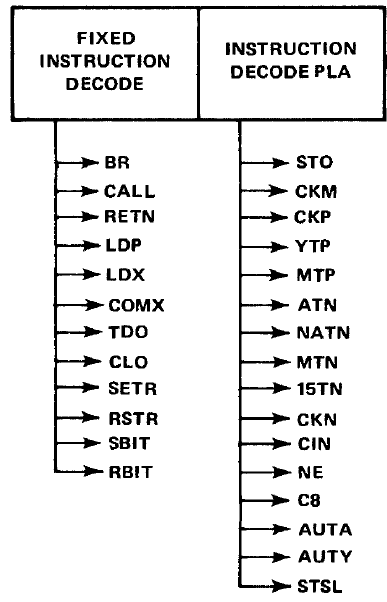
\includegraphics[scale=0.3]{images/IDEC.PNG}
			\end{column}
			\begin{column}{5cm}
				\begin{itemize}
					\item 12 feste Instruktionen \pause
					\item 31 programmierbare Instruktionen \pause
					\item Sind standardm{\"a}{\ss}ig definiert, k{\"o}nnen aber abge{\"a}ndert werden \pause
					\item PLA kombiniert die 16 Mikroinstruktionen zu einem Ausdruck
				\end{itemize}
			\end{column}
		\end{columns}
\end{frame}


\begin{frame}
\frametitle{Aufbau \& Funktionsweise}
	\framesubtitle{INIT-Pin}
		\begin{itemize}
			\item Initialisiert die Hardware \pause
			\item Resettet PA, PC und die R- \& O-Output Register
		\end{itemize}
\end{frame}


\begin{frame}
\frametitle{Aufbau \& Funktionsweise}
	\framesubtitle{Befehlssatz}
		\begin{figure}
			\centering
				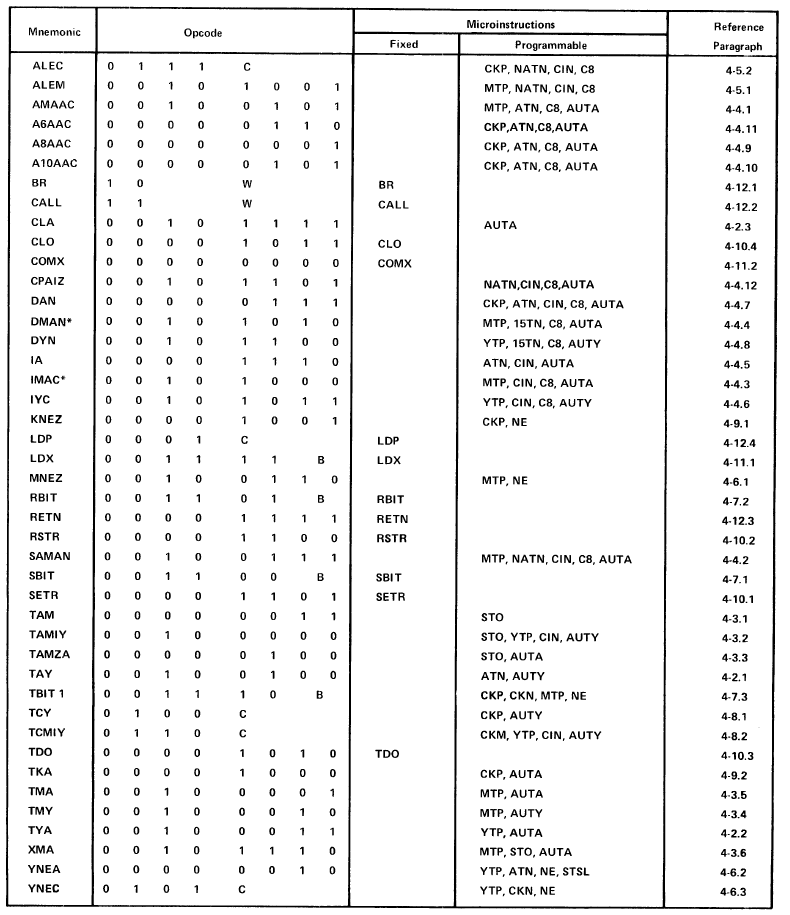
\includegraphics[scale=0.25]{images/INSTRUCT.PNG}
		\end{figure}
\end{frame}


\begin{frame}
\frametitle{Aufbau \& Funktionsweise}
	\framesubtitle{Instruktions-Formate}
		\begin{center}
			Format 1: \\
			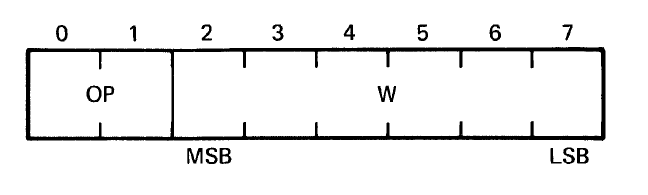
\includegraphics[scale=0.25]{images/I1.PNG} \\ \pause
			Format 2: \\
			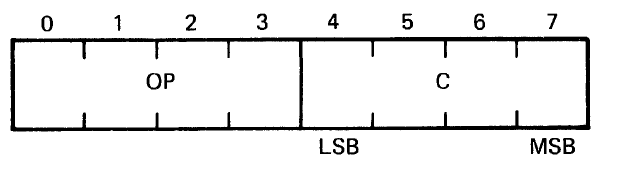
\includegraphics[scale=0.25]{images/I2.PNG} \\ \pause
			Format 3: \\
			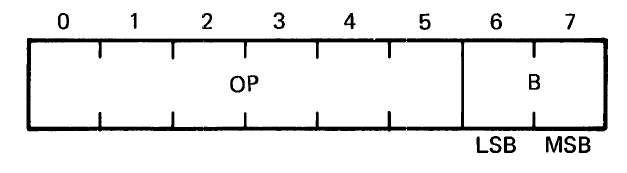
\includegraphics[scale=0.25]{images/I3.PNG} \\ \pause
			Format 4: \\
			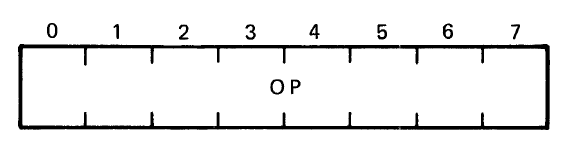
\includegraphics[scale=0.25]{images/I4.PNG} \\ 
		\end{center}
\end{frame}


\begin{frame}
\frametitle{Aufbau \& Funktionsweise}
	\framesubtitle{Beispiel: AMAAC}
		\begin{itemize}
			\item Add Memory to Accumulator, Result to Accumulator \pause
			\item Format: 4 \pause
			\item Mikroinstruktionen: MTP, ATN, C8, AUTA \pause
			\item M(X,Y) + A in A \pause
			\item Carry = 1 falls Summe gr{\"o}{\ss}er 15
		\end{itemize}
\end{frame}

\begin{frame}
\frametitle{Aufbau \& Funktionsweise}
	\framesubtitle{Beispiel: SAMAN}
		\begin{itemize}
			\item Substract Accumulator from Memory, Result to Accumulator \pause
			\item Format: 4 \pause
			\item Mikroinstruktionen: MTP, NATN, CIN, C8, AUTA \pause
			\item M(X,Y) - A in A \pause
			\item Carry = 0 falls A gr{\"o}{\ss}er M(X,Y)
		\end{itemize}
\end{frame}

\begin{frame}
\frametitle{Aufbau \& Funktionsweise}
	\framesubtitle{Beispielprogramm}
		\begin{figure}
			\centering
				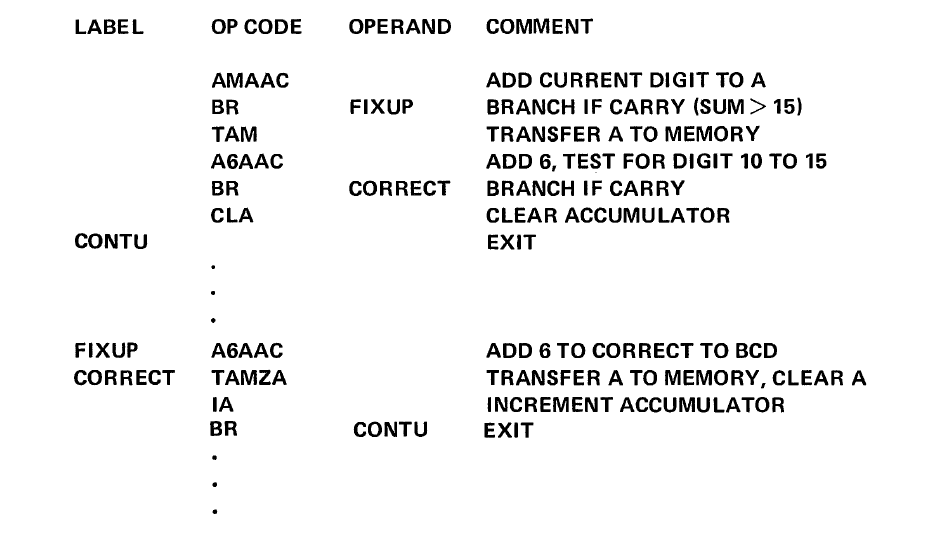
\includegraphics[scale=0.3]{images/BSPProg.PNG}
		\end{figure}
\end{frame}

\subsection{Verwendung Mikrocontroller}
\begin{frame}
	\frametitle{Verwendung}
		\begin{itemize}
			\item In eingebetteten Systemen \pause
			\item In Leistung und Austattung meist auf eine Anwendung angepasst \pause
			\item Beispiele: Unterhaltungselektronik, Waschmaschinenen, Steuerger{\"a}te, uvm. \pause
			\item TMS1000: Taschenrecher, wie z.B SR-16
		\end{itemize}
\end{frame}

\begin{frame}
\frametitle{Verwendung}
	\framesubtitle{Der SR-16}
	\begin{columns}
		\begin{column}{5cm}
			\centering
				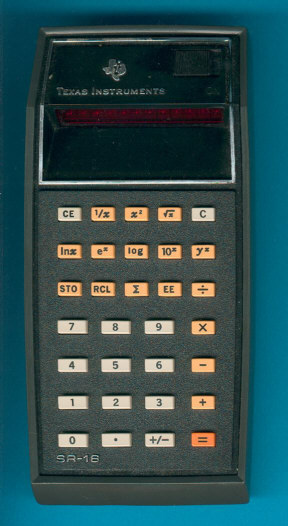
\includegraphics[scale=0.3]{images/sr-16.jpg}
		\end{column}
		\begin{column}{5cm}
			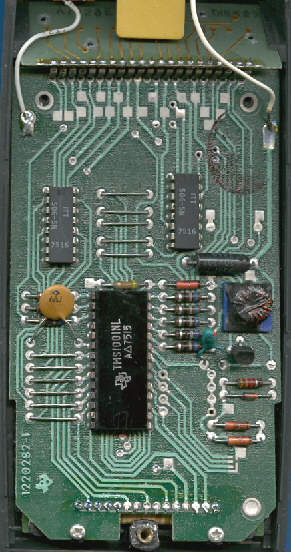
\includegraphics[scale=0.4]{images/SR-16_PCBC.jpg}
		\end{column}
	\end{columns}
\end{frame}		

	\chapter{Schluss}
\newpage
Test Schluss
\end{spacing}
\newpage
\thispagestyle{empty}
\null

\newpage
\addcontentsline{toc}{chapter}{List of figures}
\listoffigures

%\input{appendices}

\newpage
\thispagestyle{empty}
\null
	
% Generierung des Literaturverzeichnisses
%\bibliography{/path/to/your/.bib/file}

\end{document}
